% !TEX root = ../main.tex
\chapter{Diagnosis Algorithm} \label{ch:diagnosis}
In this chapter will be outlined the diagnosis algorithm\cite{semantic_diagnoser} developed by IBM Research with the collaboration of Michael Maghella, a fellow student at Università degli Studi di Brescia. This algorithm is based on a novel reputation-based approach that makes use of the informations available in the semantic graph to identify cause-effect relationships and use these relationships to isolate relevant causes basing the diagnosis on the time series data.
\section{General description}
The diagnosis activity is comprised of three main steps:
\begin{itemize}
  \item fault detection, that is the discovery of the fault. A diagnoser needs to be able to tell apart the normal behaviours from faulty ones. This is done, in this approach, through the rules discovered while learning the normal behaviour of a building (see \autoref{subsec:learn_behaviour}). Whenever a fault is detected the diagnosis process ought to start.
  \item fault isolation, that is the discovery of the causes of the fault. It is a key step for enabling a precise diagnosis of the problem. In this approach informations derived from the semantic graph are used to narrow down the set of possible faults to the most relevant ones.
  \item fault identification, that is to determine with some confidence which are the actual causes of a fault among all the possible causes. The proposed diagnoser implements a voting scheme to identify these causes.
\end{itemize}
While explaining the diagnosis approach, it will be used the same model presented in \autoref{ch:model} ( \autoref{fig:ex_building_full}), that will be represented in a compact notation shown in \autoref{fig:simple_model}, where every component is an instance of a concept with the same name (internalized representation). Moreover, for the sake of simplicity, the physic model of the system is simplified to a more lax one, dropping the MISO processes and the PT1 ones in favor of the PP and NP ones.
\begin{figure}
  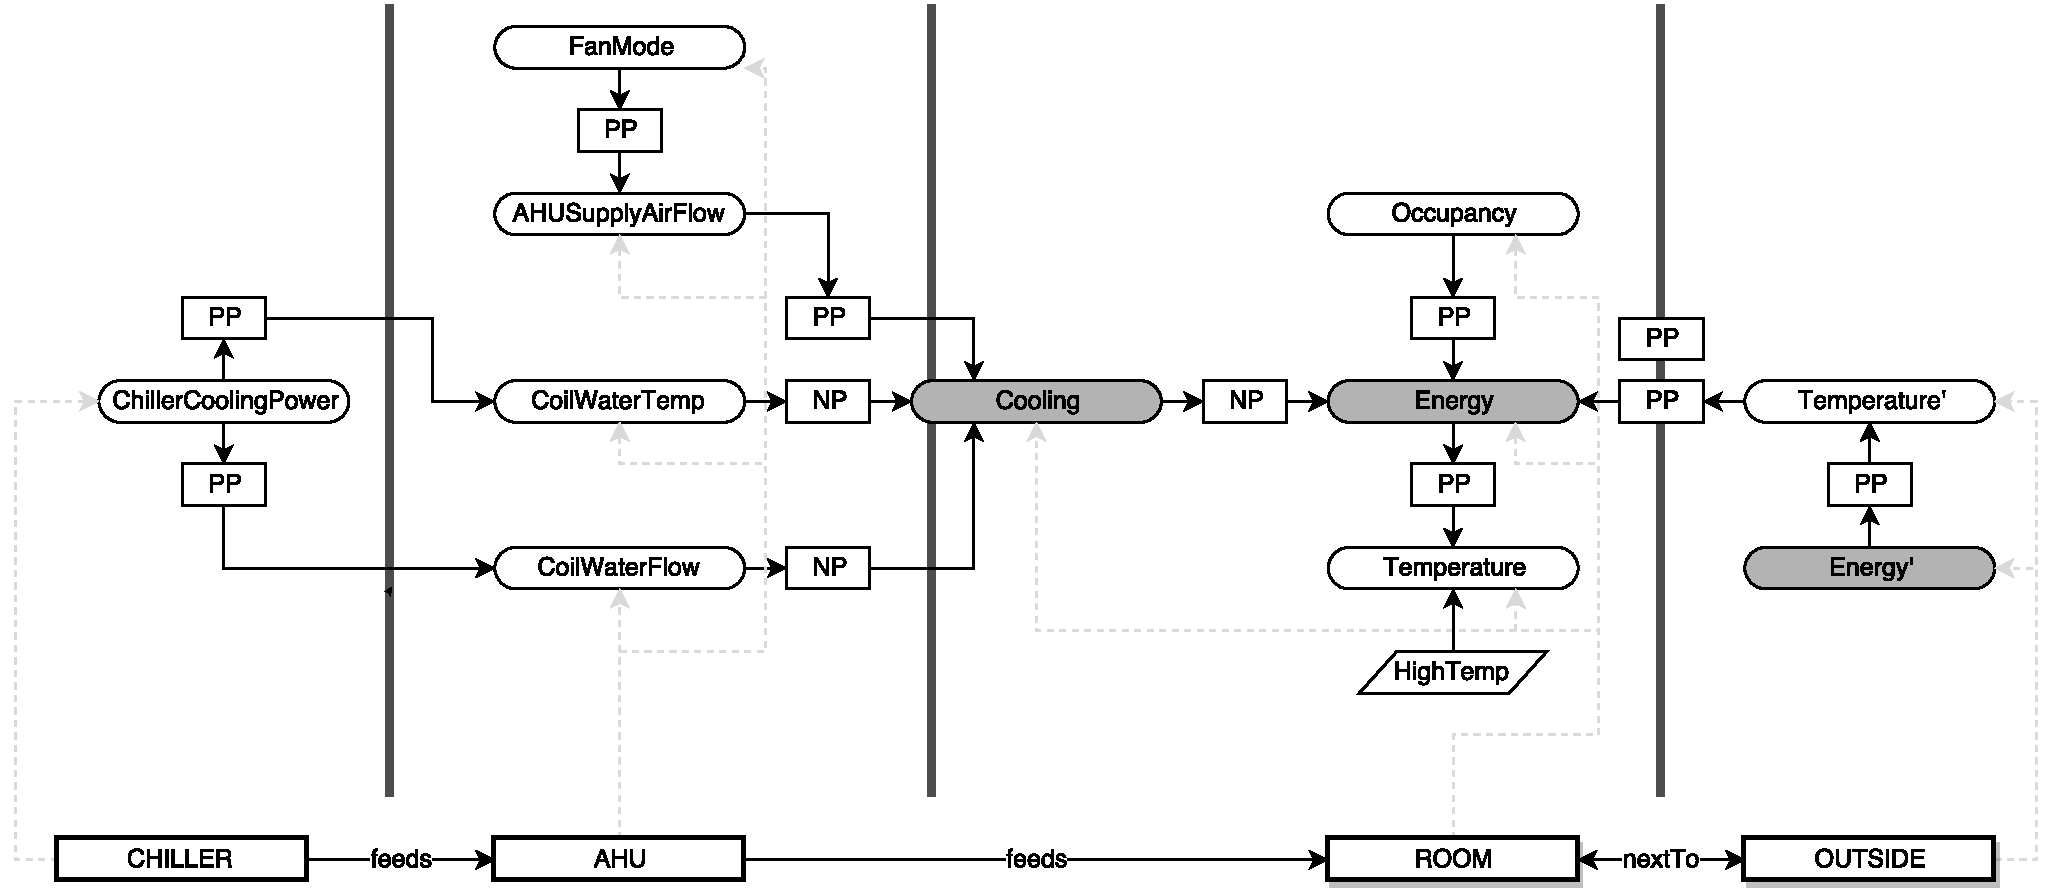
\includegraphics[width=\textwidth]{simple_diagnosis_ex.pdf}
  \caption{Internalized model of the example building}
  \label{fig:simple_model}
\end{figure}
The diagnoser is run every time an anomaly is detected in the time series. An anomaly is intended as a deviation from the normal behaviour clearly detectable by some preset upper and lower bounds, therefore an anomaly can be classified as High or Low.
It is assumed that an anomaly is symptom of some kind of fault in the system. The algorithm starts, as soon as the anomaly is detected, by identifying the semantic type of the anomaly and the potential causes in the graph. It proceeds computing the voting vector and, eventually, it is recursively executed for all those properties that get a voting score equals or greater then one. When no other causes with a high score are left, the algorithm terminates and produces a list of the detected causes along with the name of the faulty properties, the semantic type of the faults and the estimatation, expressed in percentage, of the responsability of those causes towards the diagnosed anomaly. The relative pseudocode is in \autoref{alg:diagnosis_algorithm}.
\begin{algorithm}
  \caption{General diagnosis algorithm}\label{alg:diagnosis_algorithm}
  \begin{algorithmic}[1]
    \Require
      \Statex the anomaly $A$,
      \Statex the semantic graph $\mathcal{G}$
    \Ensure a set $C_A$ of possible causes of the anomaly
    \Procedure{diagnoseAnomaly}{$A,\mathcal{G}$}
    \State $T\leftarrow$ \Call{getSemanticTypeOfAnomaly}{$A$}
    \State $PC_A\leftarrow$ \Call{getPossibleCausesInGraph}{$A,T,\mathcal{G}$}
    \State $C_A\leftarrow\emptyset$
    \State $\bm v\leftarrow$ \Call{computeReputationVoteVector}{$A,T,PC_A$}
    \ForAll {$p\in PC_A$}
    \If{$\bm v[p]\geq 1$}
    \State $C_p\leftarrow$ \Call{diagnoseAnomaly}{$p,\mathcal{G}$} \Comment{diagnose subtree}
    \If{$C_p\neq\emptyset$}
    \State $C_A\leftarrow C_A\cup C_p$
    \Else
    \State $C_A\leftarrow C_A\cup\{p\}$ \Comment{$p$ is a root cause}
    \EndIf
    \EndIf
    \EndFor
    \EndProcedure
  \end{algorithmic}
\end{algorithm}
\section{Potential causes}\label{sec:potential_causes}
The first non-trivial operation of the algorithm is the identification of the possible causes of a given anomaly. A potential cause is an observation made by a sensor that observes a property and such that the following hold:
\begin{enumerate}
  \item the property observed by the sensor is an input of a process that directly outputs to the anomaly, or it is connected to the anomalous property by a chain of unobservable properties
  \item it is observable.
\end{enumerate}
The properties and their relationships with the anomaly are all encoded in the semantic graph and are therefore accessible via reasoning. The approach is also interested in the semantic type of the anomaly and of the possible causes.
Retrieving the possible causes of an anomaly is possible because in the graph anomalies are observations made by a sensor that measures a property.
\begin{figure}
  \begin{subfigure}[b]{\textwidth}
    \centering
      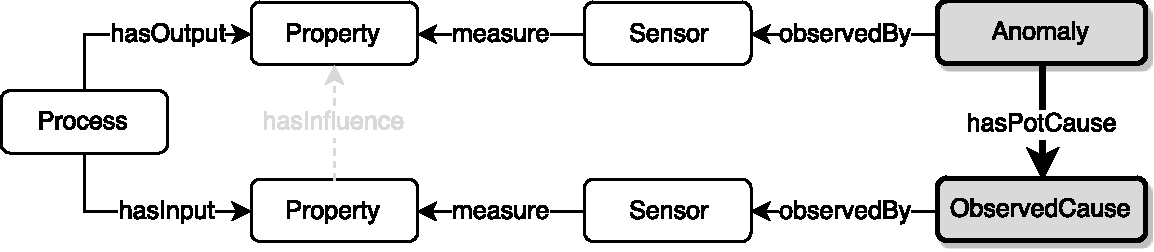
\includegraphics[width=.9\linewidth]{direct_cause.pdf}
      \caption{Direct influence}
      \label{fig:direct_influence}
  \end{subfigure}
  \bigskip
  \begin{subfigure}[b]{\textwidth}
    \centering
      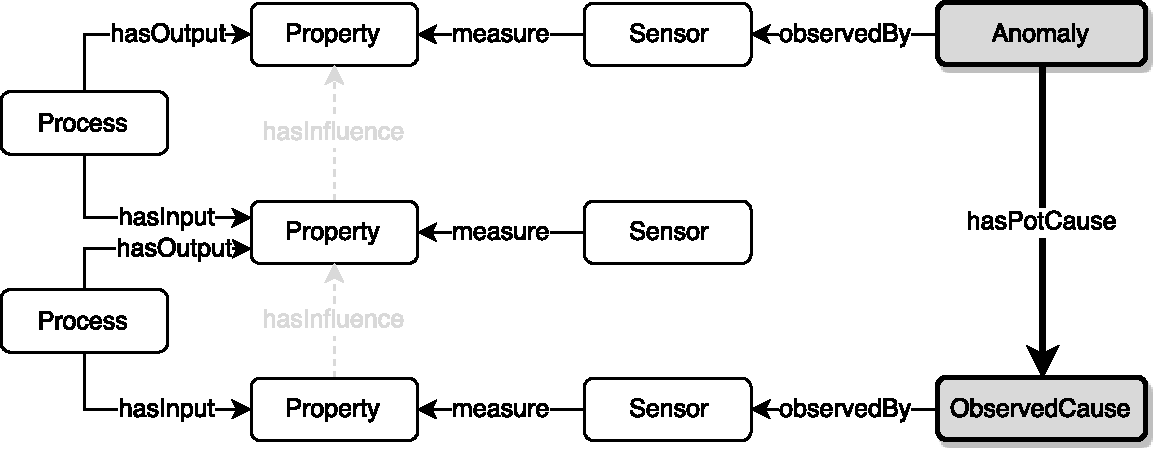
\includegraphics[width=.9\linewidth]{unobs_chain.pdf}
      \caption{Chain of unobservables properties}
      \label{fig:chain_unobs}
  \end{subfigure}
  \caption{Detection of potential causes}
  \label{fig:pot_causes}
\end{figure}
\autoref{fig:pot_causes} shows the possible ways to retrieve a potential cause of a property. In both graphs the situation respects the conditions given earlier regarding potential causes.
The causes retrieved at this point are the ones that are correlated at various degrees to the anomaly and are the only ones that can help to produce a diagnosis. At this point it is important to preserve the semantic informations %TODO drop ``s'' from information in every chapter
about the processes involved since these informations are at the base of the voting algorithm. When talking about ``semantic informations'' of the process it is meant the replacement of a chain of properties with a single, direct process whose type is infered from the ones of the chain. For example it can be seen in \autoref{fig:chain_composition} that the temperature in a room is influenced by the occupancy property of the room through a chain of a PT1 process and a PP process, both involving the unobservable energy property. This means that the temperature is influenced by the occupancy through a direct PT1 process.
\begin{figure}
  \centering
  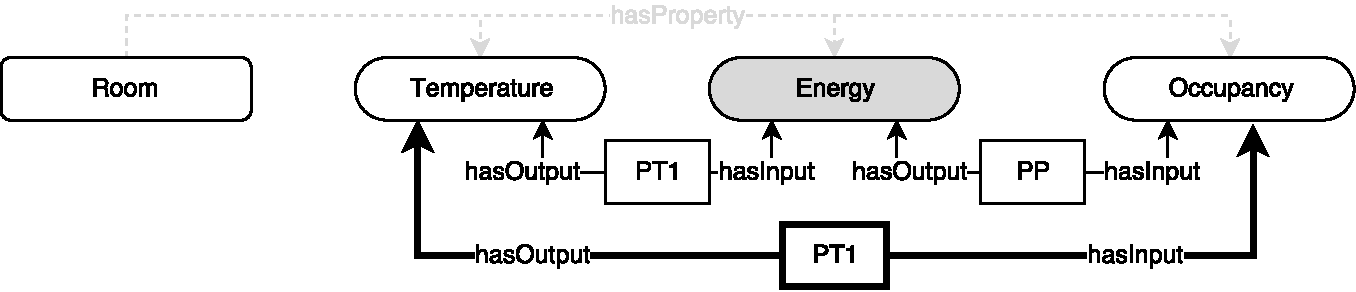
\includegraphics[width=1\textwidth]{process_chaining.pdf}
  \caption{Process chain composition}
  \label{fig:chain_composition}
\end{figure}
\autoref{tab:process_chains_combination} shows the possible combinations for the most common type of processes used that are the positive correlation, the negative correlation and the lag processes.
\begin{table}
  \centering
  \caption{Derived processes from most common process chains}
  \label{tab:process_chains_combination}
  \begin{tabular}{lll}
    \hline\textbf{First process} & \textbf{Second process} & \textbf{Derived process}\\\hline
    Positive correlated & Positive correlated & Positive correlated\\
    Positive correlated & Negative correlated & Negative correlated\\
    Negative correlated & Positive correlated & Negative correlated\\
    Negative correlated & Negative correlated & Positive correlated\\
    Any & Lag & Lag \\\hline
  \end{tabular}
\end{table}
Given these new processes that directly correlate an anomaly to its potential causes, it is possible to infer the entity of the potential cause. This information is computed thanks to the intuition that the type of process correlating two observation carries qualitative information about the output. It is possible to predict that an observation has to be high if it is influenced by a positive correlation process whose input is an observation that is high itself. The ontology defines the combinations listed in \autoref{tab:anomaly_type_prediction}.
\begin{table}
  \centering
  \caption{Predicted value of an observation given the influencing process and its input}
  \label{tab:anomaly_type_prediction}
  \begin{tabular}{lll}
    \hline\textbf{Anomaly type} & \textbf{Process type} & \textbf{Cause type}\\\hline
    High & Positive correlated & High\\
    High & Negative correlated & Low\\
    Low & Positive correlated & High\\
    Low & Negative correlated & Low \\
    Any & Lag & Lag \\\hline
  \end{tabular}
\end{table}
Thanks to those informations it is possible to implement the fault identification capablities of the algorithm.
\section{Fault identification}
The whole approach is based on the intuitive assumption that an anomaly is caused by faults and that the measurement of the behaviour of such faults needs to be anomalous too. Moreover this anomalous behaviour needs to be semantically coherent with the behaviour predicted from the chain of process that links the anomaly to the cause. These two principles are at the base of the voting algorithm.
\begin{algorithm}
  \caption{Voting algorithm}\label{diagnosis}
  \begin{algorithmic}[1]
    \Require
      \Statex the anomaly $A$,
      \Statex a set of possible causes of $ A, PC_A$,
      \Statex the semantic type of the anomaly, $T$,
    \Ensure the vector of votes, $\bm v$
    \Procedure{computeReputationVoteVector}{$A,T,PC_A$}
    \State $S\leftarrow$ \Call{getHistoricaltime series}{}
    \State $S'\leftarrow$ \Call{getSimilarHistoricalData}{$S,A$}
    \State $\bm V\leftarrow\emptyset$\Comment{the voting matrix}
    \ForAll {$p\in PC_A$}
    \State $S''\leftarrow$ \Call{getSimilarHistoricalData}{$S',p$}
    \ForAll {$c\in PC_A$}
    \State $d_{p,c}\leftarrow$ \Call{calculateDistance}{$S'',c$}
    \State $v_{p,c}\leftarrow$ \Call{calculateDistance}{$S'',c$}
    \EndFor
    \State $\bm r\leftarrow$ \Call{calculateReputation}{$\bm V$}
    \State $\bm v\leftarrow$ \Call{weightVotes}{$\bm V, \bm r$}
    \EndFor
    \EndProcedure
  \end{algorithmic}
\end{algorithm}
The algorithm works by computing, from the set of anomaly-free time series, a world view (that is a subset of the historical data for each time series) where the property that presents an anomaly would be anomaly-free but close in range to the anomalous value. This can be done by selecting all the anomaly-free data of the sensor that observes the fault; these values are splitted in deciles and the decile closest to the anomalous value is chosen, that is the first decile if the anomaly is of type Low or the tenth if it is of type High. For every potential cause are then extracted the samples measured at the same timestamp as the samples of the anomalous property that fall in the chosen decile.
\begin{figure}
  \centering
  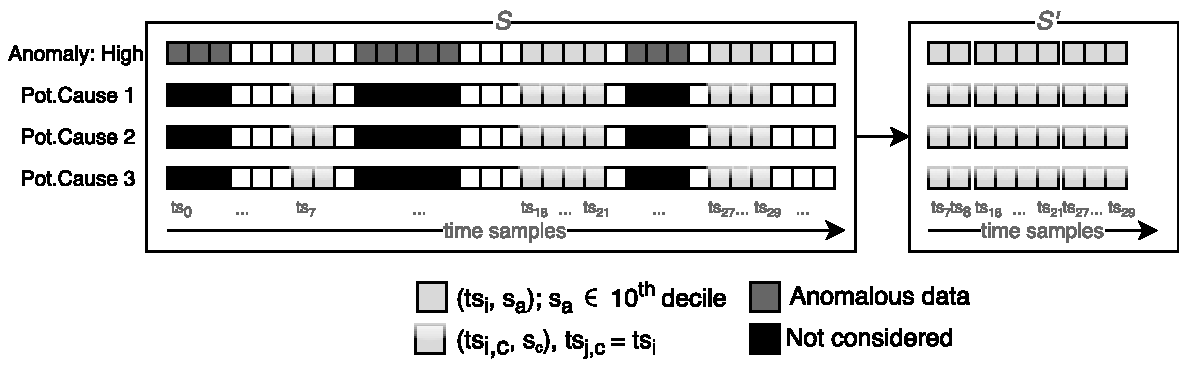
\includegraphics[width=\textwidth]{subset_creation.pdf}
  \caption{Creation of the set $S^{'}$}
  \label{fig:subsets}
\end{figure}
Given this subset $S^{'}\subset S$, each potential cause will derive a second subset $S^{''}_p\subset S^{'}$ which represents the view of the system from the point of view of one of the potential causes, that provide its point of view assuming it is not anomalous itself. The method is the same described for the computation of $S^{'}$, using the value observed for that property at the time of the anomaly instead of the one of the anomaly itself.
At this point every potential cause $p$ has the informations needed to give the opinion, that is to vote, about which is the actual cause $c$ of the fault, according to its perceived state of the world $S^{''}_p$. The voting is expressed in terms of normalized mean distance $d_{p,c}$ between the actual value, observed by the suspect property $c$ at the time $t_0$ of occurence of the anomaly, and the mean of the samples values that represents the behaviour of the potential cause expected by the voting variable.
\begin{equation}
  \label{eq:norm_mean_dist}
  d_{p,c}=10\frac{s_c(t_0)-\operatorname{mean}S^{''}_{p,c}}{\operatorname{max}S_c-\operatorname{min}S_c}
\end{equation}
\textcite{semantic_diagnoser} suggests a modification to \autoref{eq:norm_mean_dist} in order to tackle scenarios involving delays. This modification leads to
\begin{equation}
  \label{eq:delayed_distance}
  \begin{gathered}
  d_{p,c}=10\frac{\operatorname{mean}(\sum_{\tau=0}^{\tau_{U}}s_c(t-\tau))-\operatorname{mean}S^{'''}_{p,c}}{\operatorname{max}S_c-\operatorname{min}S_c}\\
  \text{with }S^{'''}=\{s_c(t^{'''}\in S_c^{''}|t^{'''}\leq t-\tau_U\}
\end{gathered}
\end{equation}
so that all relevant previous values up to a maximum delay are taken into account and their mean value is used instead of the value at the time of the anomaly. The expected comparison value is calculated over a subset $S^{'''}$ including only samples before $t-\tau_U$ so that values that are in the scope of the delay are not used as comparison values.
Normalization occurs in a range of [-10,10] with the maximum and minimum value of the whole time series in $S$ (anomalous values included). These steps ensure that the different measurements can be comparable.
The resulting distance is less then zero if the actual value observed for a property is lower than the value the voting property is expecting to see, it is greater than zero otherwise. This information about the signedess of the computed distance plays a key role during the fault identification because it helps discriminating between anomalous values that are the cause of a fault and those anomalous values that are effect of a fault. That means that if the behaviour of a property doesn't match the behaviour that a cause should have, said property can't be a cause and its vote is set to zero.
\begin{equation}
  \label{eq:vote}
  v_{p,c}=\begin{cases}
    d_{p,c} & \text{if } d_{p,c}\geq 0 \land \operatorname{type}c\equiv High \\
    -d_{p,c} & \text{if } d_{p,c}\leq 0 \land \operatorname{type}c\equiv Low \\
    \left\lVert d_{p,c}\right\rVert & \text{if } \operatorname{type}c\equiv Unknown \\
    0 & \text{otherwise}
\end{cases}
\end{equation}
For example, if a room's temperature is too high and the real faulty property is the outside temperature, there's a chance that the chiller power consumption will be anomalous too since the chiller is trying to mitigate the effect of the fault. Still the chiller is not the cause of the anomaly. Once the computation of the distances ends, the matrix of the votes is filled with the ``opinions'' that the potential causes have about each other. Since the votes have been calculated under the assumption that the potential cause that is voting is under normal circumstances, if said cause is the origin of the fault then it will flag as faulty all the others because its point of view will be so distorted that normal behaviours appear as anomalous. This tendency of faulty properties is misleading for the diagnoser and thus needs to be addressed. The way this algorithm deals with the problem is through the means of the concept of reputation. A potential cause has a high reputation $r_p$, hence it is trustworthy, if it doesn't receive any vote from other causes. The reputation decreases as the property receives more votes, as seen in \autoref{eq:reputation}.
\begin{equation}
  \label{eq:reputation}
  r_p=\frac{1}{1+\sum\limits_{c\in PC_A}v_{p,c}}
\end{equation}
Given the reputation vector $\bm r=\{r_i|i\in PC_A\}$, the total vote $v_p$ received by a potential cause $p$ is given by the sum of the votes of all the properties weighted by the reputation of the property that gave that vote (\autoref{eq:weighted_vote}). It is considered abnormal every property that has a value higher then 1.
\begin{equation}
  \label{eq:weighted_vote}
  v_p=\sum\limits_{c\in PC_A}r_c\cdot v_{p,c}
\end{equation}
An alternative kind of vote is the so called vote count. This method drops the magnitude of the votes and simply counts how many votes greater than one have been assigned to a given property $p$. (\autoref{eq:vote_count}).
\begin{equation}
  \label{eq:vote_count}
  \begin{gathered}
  \bar v_p=\sum\limits_{c\in PC_A}\operatorname{discretize}{(r_c\cdot v_{p,c})}\\
  \operatorname{discretize}{x}=\begin{cases}
      1 & \text{if } x\geq 1\\
      0 & \text{otherwise}
    \end{cases}
  \end{gathered}
\end{equation}
The formulae result in the vote vectors $\bm v=\{v_p|p\in PC_A\}$ and $\bm{\bar v}=\{\bar v_p|p\in PC_A\}$.
Using one method or the other yelds different results and which one to use is decided upon execution on a per-case basis. Experiments \cite{semantic_diagnoser} demonstrated that it is usually better to use the vote count whereas there could be multiple faults.
\section{Diagnosis example}
In this section it is shown how the diagnosis takes place in the context of a building as in \autoref{fig:simple_model}. It is assumed that data picked up by the sensors just before the anomaly occurs are distributed as in \autoref{fig:timeseries}. The rule that monitors the anomaly is ``if the room's temperature is greater than \ang{25} there's an anomaly'' and the fault is due to the chiller that stopped to work at 1 pm.
\begin{figure}
  \centering
  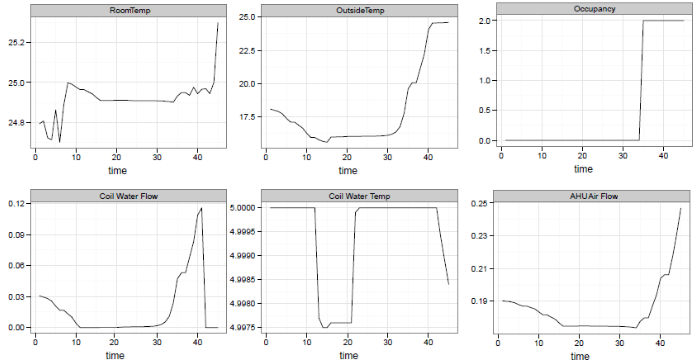
\includegraphics[width=1\textwidth]{timeseries.png}
  \caption{Example of time series of different sensors}
  \label{fig:timeseries}
\end{figure}
The room temperature starts rising and a first anomaly is detected, thus starting the diagnosis process.
Since the anomaly is a temperature greater than \ang{25}, the semantic type of the anomaly is High. Then the possible causes can be traced back, following the rules explained above. The anomaly is detected because of the room temperature and so the properties connected to that property are traced back. The room temperature is influenced by the internal energy of the room, that is unobservable. This violates the second rule and so energy can't be a potential cause and needs to be resolved. This leads to discover as potential causes the occupancy, that is a potential cause via a positive proportional process (see \autoref{tab:process_chains_combination}), the outside temperature, still via a positive proportional process, and the cooling property. Once again, cooling property is unobservable and needs to be traced back.
All the backtracked causes and the derived processes are shown in bold in \autoref{fig:backtracking_example}.
\begin{figure}
  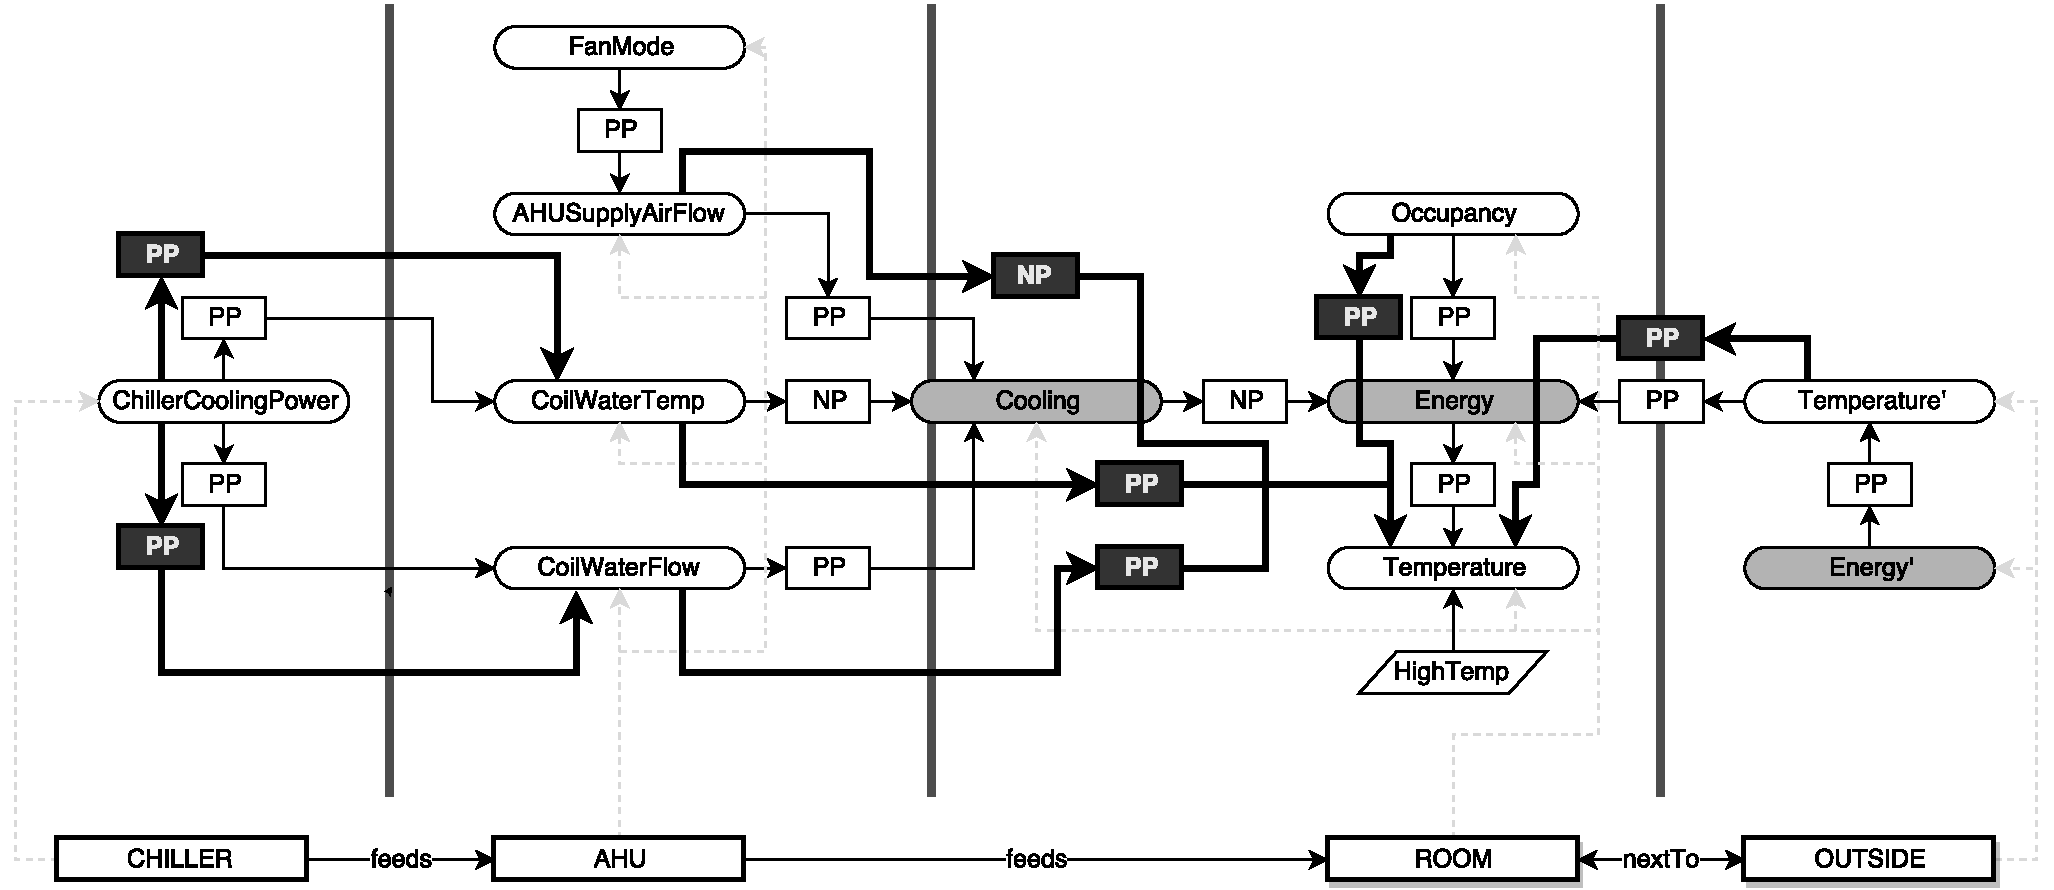
\includegraphics[width=1\textwidth]{backtrack_example.pdf}
  \caption{Backtracking the possible causes of a HighTemp anomaly}
  \label{fig:backtracking_example}
\end{figure}
As soon as the potential causes are known, it is possible to predict the semantic value of said causes and according to \autoref{tab:anomaly_type_prediction} it is derived the graph shown in \autoref{fig:semantic_type}.
\begin{figure}
  \centering
  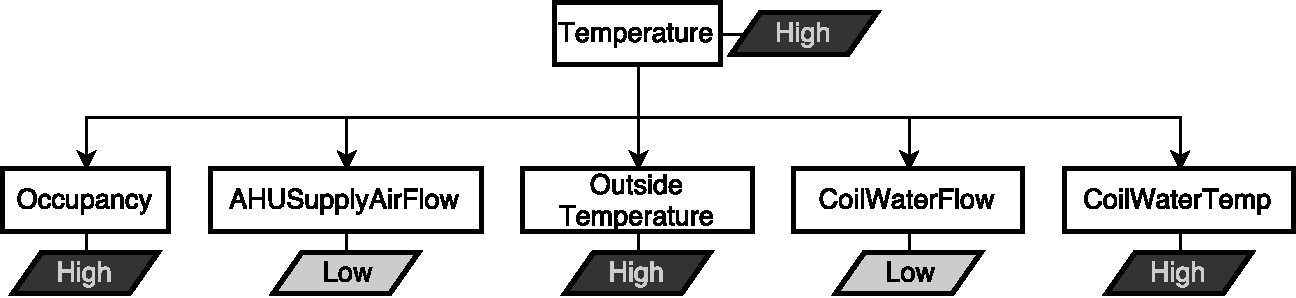
\includegraphics[width=.8\textwidth]{infer_semantic_type.pdf}
  \caption{Semantic type of potential causes}
  \label{fig:semantic_type}
\end{figure}
The diagnoser has enough informations for computing the vote vector. It starts from collecting the time series measured by the sensors observing the involved properties (\autoref{fig:timeseries}) and thus populating the $S$ set.
From this set the diagnoser tries to extract the subset $S^{'}\subset S$. This is done by extracting the anomaly-free historical time series and by computing the deciles over these data. Since the anomaly was of type High, it is selected the tenth decile ranging from \ang{24.86}C to \ang{25}C. The time series of other properties involved are derived by sampling the property time series at each timestamp such that at that time the room temperature is between \ang{24.86}C to \ang{25}C. This set $S^{'}$ represents the normal behaviour of the building that is closer to the anomalous one and is the common ground used by every potential cause to build its own point of view. Each potential cause $p$ can use this common ground to derive a subset $S_p^{''}\subset S^{'}$ based on the similarity respect to the value of the property at the time of the anomaly.
\begin{figure}
  \begin{subfigure}[b]{.5\textwidth}
    \centering
      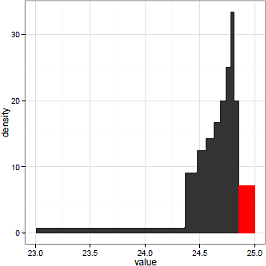
\includegraphics[width=.9\linewidth]{deciles_room.png}
      \caption{Deciles computed for anomalous property}
      \label{fig:room_deciles}
  \end{subfigure}
  ~
  \begin{subfigure}[b]{.5\textwidth}
    \centering
      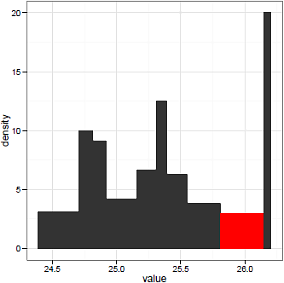
\includegraphics[width=.9\linewidth]{deciles_out.png}
      \caption{Deciles computed for outside temperature}
      \label{fig:out_deciles}
  \end{subfigure}
  \caption{Deciles ranges used for computation of $S^{'}$ and $S^{''}$}
  \label{fig:deciles}
\end{figure}
Once the subsets are derived, the properties can express their vote.
The vote matrix is shown in \autoref{tab:vote_matrix}. It is interesting to note how the supply air flow property doesn't get any vote even if its value is abnormally increasing after the anomaly, as see in \autoref{fig:timeseries}. This is due to the fact that the system expects the supply airflow to be lower than the usual for it to be a cause of the fault. The AHU tries to make up for the fault at the chiller by increasing the air flow to cool the room, hence it is a ``good'' behaviour. Since the supply air flow property contradicts the behaviour that a cause should have, it can't be a cause and its vote is set to zero according to \autoref{eq:vote}. In \autoref{tab:vote_matrix} is also shown the property reputation calculated as in \autoref{eq:reputation}.
\begin{table}
\centering
\caption{Vote matrix}
\label{tab:vote_matrix}
\begin{tabular}{l|lllll}
& \textbf{Occ} & \textbf{CWT} & \textbf{SAF} & \textbf{CWF} & \textbf{OT} \\\hline
\textbf{Occupancy} & 0  & 0.0010       & 0            & 3.741        & 1.437       \\
\textbf{CoilWaterTemp}      & 0.909        & 0            & 0            & 3.331        & 1.394       \\
\textbf{SupplyAirFlow}      & 0            & 0            & 0            & 7.678        & 0.470       \\
\textbf{ChillerWaterFlow}   & 0.909        & 0.001        & 0            & 0            & 2.555       \\
\textbf{OutsideTemperature} & 1.8182       & 0            & 0            & 8.747        & 0.003\\\hline
\textbf{Vote sum}           & 3.636        & 0.002        & 0            & 23.497       & 5.861       \\
\textbf{Reputation}         & 0.215        & 0.997        & 1            & 0.04         & 0.145      \\\hline
\end{tabular}
\end{table}
According to \autoref{eq:weighted_vote} and \autoref{eq:vote_count} the vote vectors are calculated as shown in \autoref{tab:weighted_votes}.
\begin{table}
\centering
\caption{Weighted votes and vote vectors $\bm v$ and $\bm{\bar v}$}
\label{tab:weighted_votes}
\begin{tabular}{l|lllll}
& \textbf{Occ} & \textbf{CWT} & \textbf{SAF} & \textbf{CWF} & \textbf{OT} \\\hline
\textbf{Occupancy}             & 0            & 0            & 0            & 0.807        & 0.310       \\
\textbf{CoilWaterTemp}         & 0.906        & 0            & 0            & 3.322        & 1.390       \\
\textbf{SupplyAirFlow}         & 0            & 0            & 0            & 7.678        & 0.470       \\
\textbf{ChillerWaterFlow}      & 0.037        & 0            & 0            & 0            & 2.555       \\
\textbf{OutsideTemperature}    & 0.264        & 0            & 0            & 1.275        & 0           \\\hline
\textbf{Total Vote $\bm v$}      & 1.208        & 0            & 0            & 13.081       & 2.276       \\
\textbf{Vote Count $\bm{\bar v$}} & 0            & 0            & 0            & 3            & 1     \\\hline
\end{tabular}
\end{table}
The diagnoser will then diagnose those properties that are deemed to be causes and correctly traces back the root cause that is the chiller (see \autoref{fig:backtracking_example}).
\textcite{semantic_diagnoser} demonstrate that this approach has been able to adapt to delayed effects scenarios, multi faults scenarios with both unobservable and observable faults and to more complex buildings.
